\chapter{Resultados Experimentais}
\label{chap:Resultados}

% Gráficos e comentários provenientes de cada um dos experimentos.

% Resumo opcional. Comentar se não usar.
% \resumodocapitulo{Resumo opcional.}



\section{Sarsa Aproximado e Comportamentos Pré-Programados}

O treinamento de Sarsa realizado contou com 30.000 partidas utilizando a rede neural multicamadas descrita na Subseção \ref{subsec:sarsadev} e salvando os retornos obtidos em cada partida.

O gráfico da Figura \ref{fig:single-agent-sarsa-behaviors} mostra em conjunto o retorno a cada partida e a média do retorno a cada 100 partidas. É possível observar que há um tendência de subida do retorno com o passar dos episódios experienciados, porém em grande parte das partidas o agente não realizou nenhum gol, refletido pelo baixo valor da média de 100 partidas.

É interessante ressaltar o alto custo de processamento deste tipo de treinamento, por utilizar redes neurais. Dessa forma, a quantidade de amostras possíveis de serem coletadas em tempo hábil foram dramaticamente reduzidas.

A utilização de métodos aproximados posa um problema de duplo aprendizado: deseja-se aprender a política ótima enquanto se aprende a aproximar esta política ótima desconhecida por meio de uma rede neural. Esse fator contribui negativamente no tempo para convergência da política. Em métodos tabulares, apesar do maior custo de memória, esse problema é inexistente.

\begin{figure}[H]
	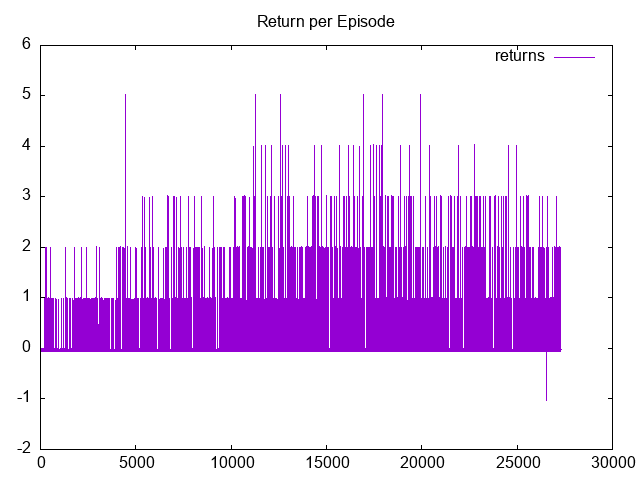
\includegraphics[width=0.9\linewidth]{figs/sarsa-tmp.png}
	\centering
	\caption{Curva de aprendizado do agente com comportamentos pré-programados utilizando Sarsa aproximado.}
	\label{fig:single-agent-sarsa-behaviors}
\end{figure}

\section{Double Q-Learning Tabular e Comportamentos Pré-Programados}

Foram executados 3 treinamentos de 100000 partidas e foram salvos a tabela Q completa e o histórico dos retornos obtidos pelo agente ao longo do treinamento.

O gráfico da Figura \ref{fig:single-agent-tabular-behaviors} mostra o histórico médio dos 3 treinamentos. Observa-se que
% o desempenho dessa abordagem supera o da abordagem anterior rapidamente, com poucas amostras. Em contrapartida, 
há uma estagnação do retorno por volta das 60000 amostras, o que pode indicar a existência de um limite superior para o desempenho do agente devido à menor flexibilidade da política aprendida ou a necessidade de ajuste no decaimento do fator de exploração para que o agente explore novas possibilidades por mais partidas.

\begin{figure}[H]
	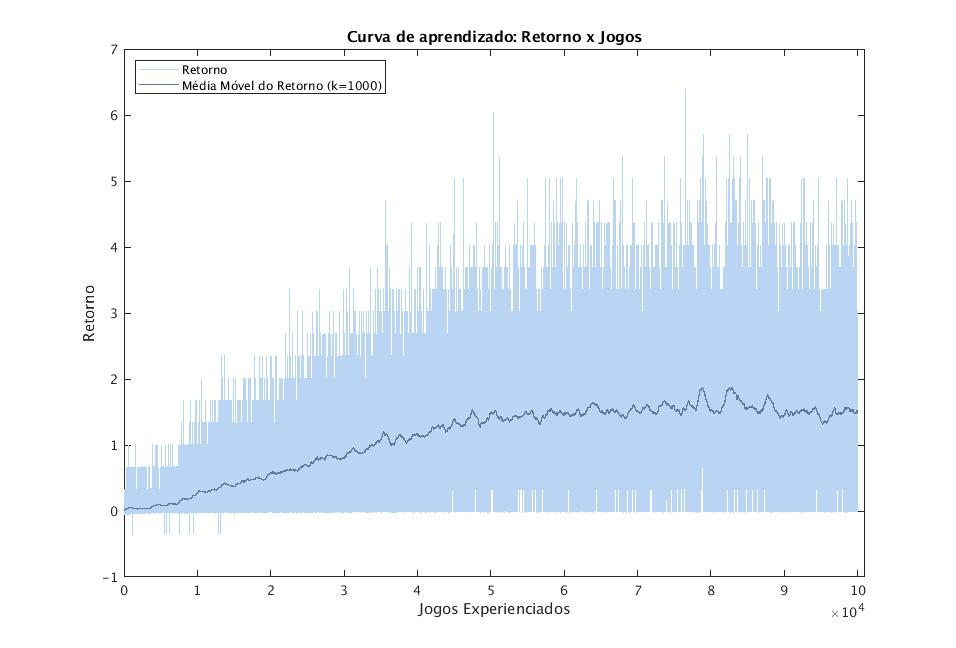
\includegraphics[width=0.9\linewidth]{figs/curva-behaviors-tabular.jpg}
	\centering
	\caption{Curva de aprendizado do agente com comportamentos pré-programados.}
	\label{fig:single-agent-tabular-behaviors}
\end{figure}

A Figura \ref{fig:goal-seq} ilustra o agente conduzindo a bola e realizando um gol conforme a política aprendida.

\begin{figure}[H]
	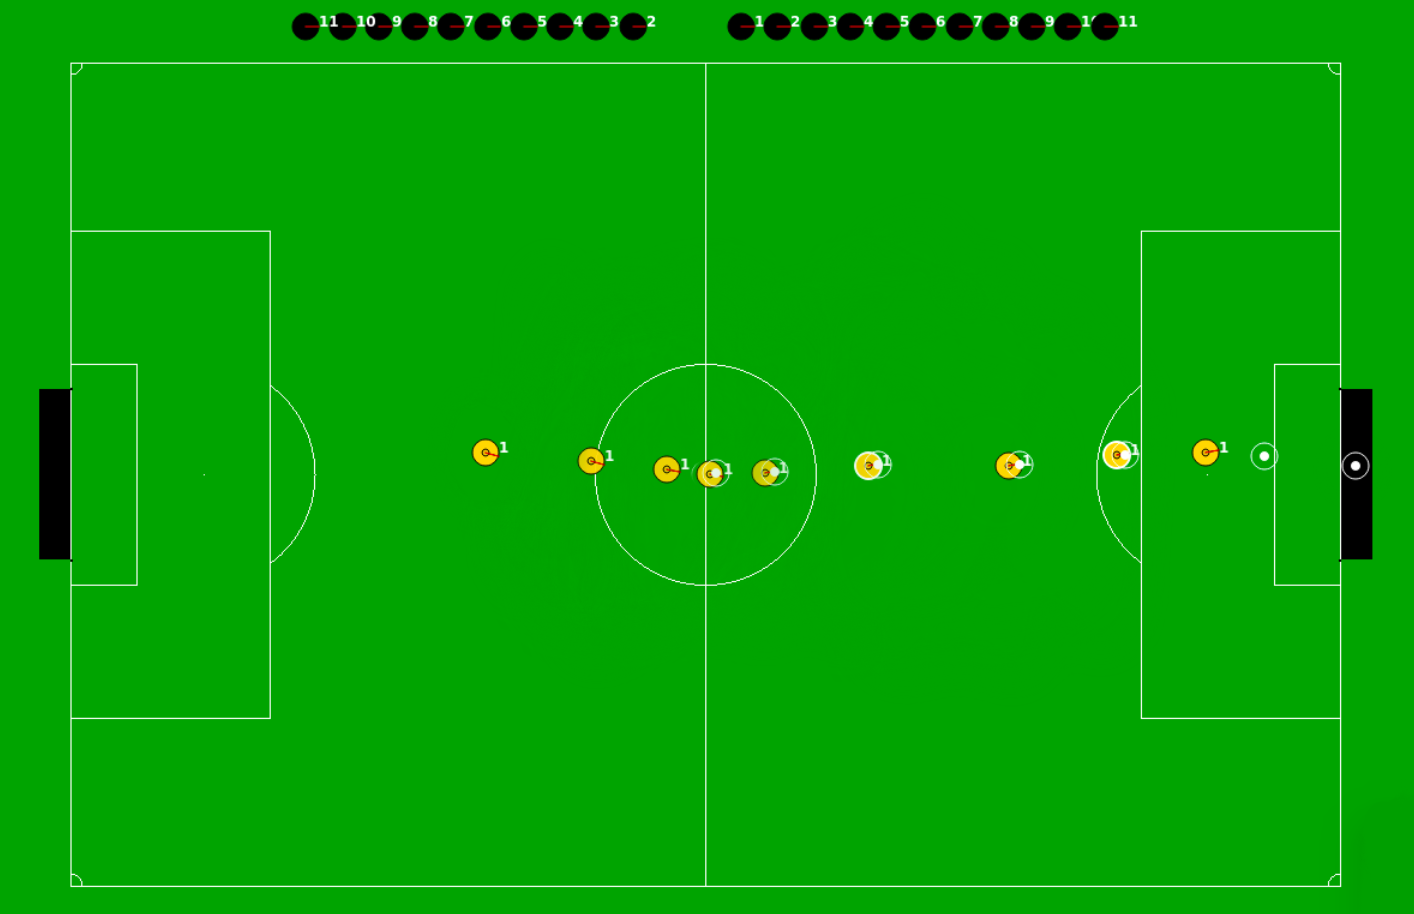
\includegraphics[width=0.9\linewidth]{figs/goal-sequence.png}
	\centering
	\caption{Sobreposição de sequência de imagens do agente fazendo gol.}
	\label{fig:goal-seq}
\end{figure}

A Figura \ref{fig:curvalonga-bhv} mostra o histórico de retornos para um treinamento mais longo, de 200000 partidas. Nela, percebe-se que após a cessação da exploração o agente estabiliza seu desempenho abaixo do máximo obtido.

\begin{figure}[H]
	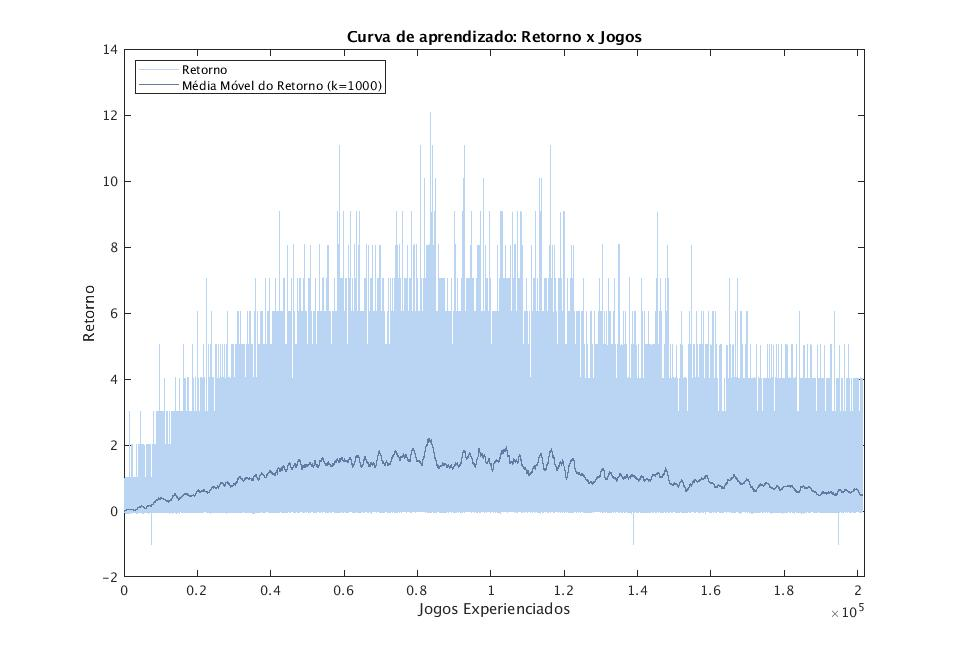
\includegraphics[width=0.9\linewidth]{figs/curvalonga-behaviors-tabular.jpg}
	\centering
	\caption{Curva de aprendizado do agente com comportamentos pré-programados para treinamento longo.}
	\label{fig:curvalonga-bhv}
\end{figure}

\section{Double Q-Learning Tabular e Ações Puras}

Foram executados 3 treinamentos distintos de 100000 partidas a fim de suavizar o elemento sorte nos resultados. Após cada um dos treinamentos foram salvos a tabela Q completa e o histórico dos retornos obtidos pelo agente ao longo do treinamento.

A Figura \ref{fig:single-agent-curva} mostra esse histórico. É interessante observar que com o decaimento dos fatores de exploração e de aprendizagem, após 100000 partidas ambos eram $\epsilon \approx 0.01648$ e $\alpha \approx 0.03679$, ou seja, o agente já executava na maior parte dos ciclos a política aprendida. Para cada jogo foi feita a média entre os 3 retornos observados em cada um dos treinamentos.

\begin{figure}[H]
	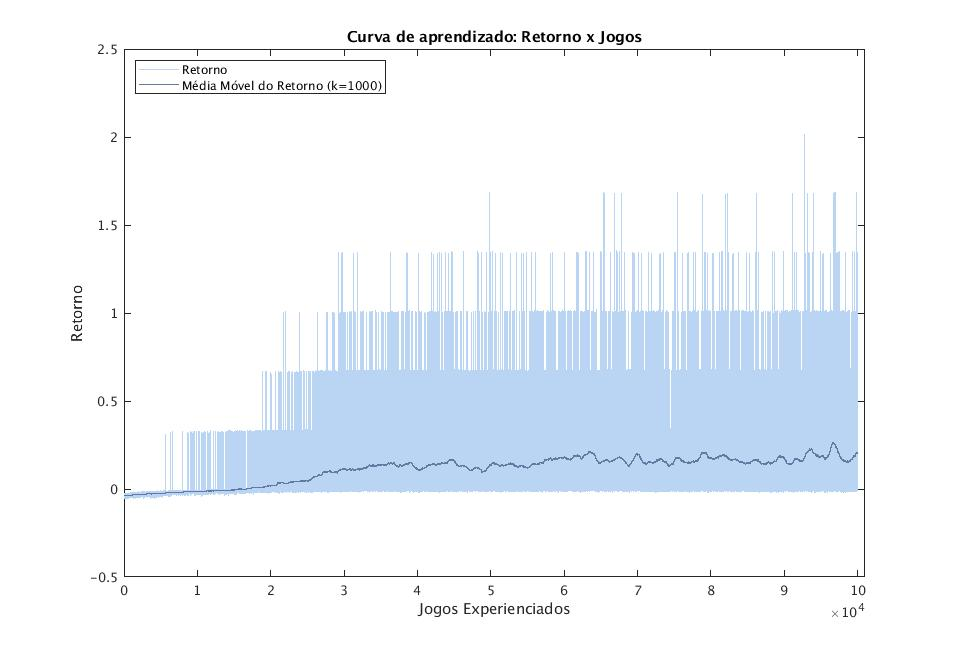
\includegraphics[width=0.9\linewidth]{figs/curva-qtabular.jpg}
	\centering
	\caption{Curva de aprendizado do agente com ações puras. }
	\label{fig:single-agent-curva}
\end{figure}

Além disso, foi executado um treinamento de 200000 partidas com os mesmos parâmetros, a fim de observar a aprendizagem por um período mais longo. Na Figura \ref{fig:single-agent-curvalonga}, observa-se a cessação de aprendizado com o decaimento do fator de exploração.

\begin{figure}[H]
	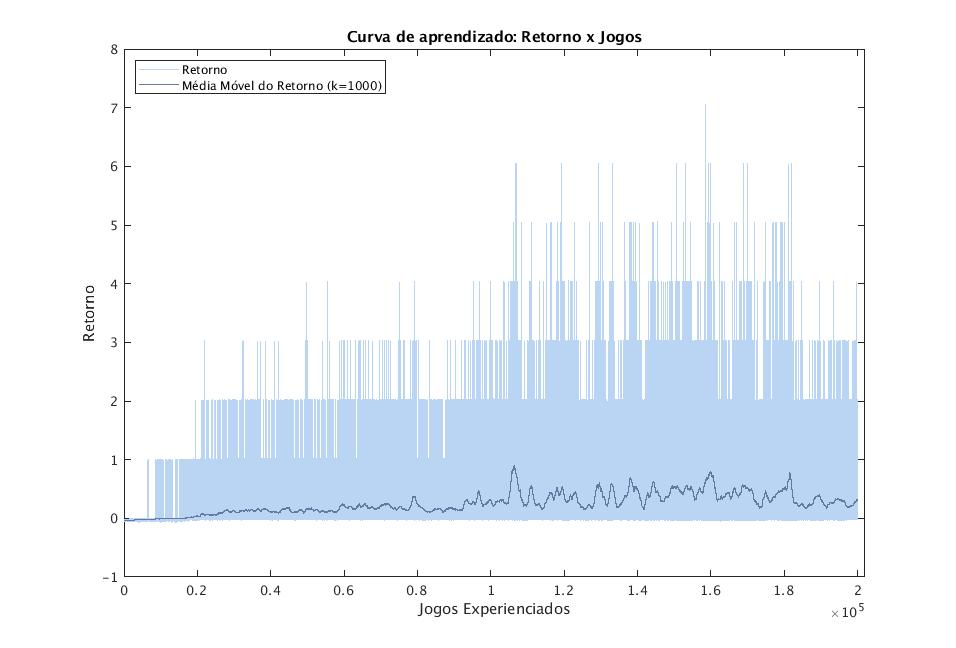
\includegraphics[width=0.9\linewidth]{figs/curvalonga-qtabular.jpg}
	\centering
	\caption{Curva de aprendizado para treinamento longo.}
	\label{fig:single-agent-curvalonga}
\end{figure}

Apesar da grande quantidade de experiência a que o agente teve acesso, nota-se na Figura \ref{fig:single-agent-curvalonga} que o crescimento de seu desempenho é bastante limitado, sequer atingindo a média de 1 gol por partida. Isso é um indicativo do altíssimo custo computacional de soluções \textit{end-to-end} como a utilizada no experimento.



% \section{Agentes Concorrentes}

% Após validação do sistema com agente único, é interessante experimentar com treinamento adversarial de apenas 2 jogadores em formato um-contra-um. A intenção dessa etapa é experimentar com o sistema o caso adversarial, no qual há um ou mais agentes com objetivo oposto ao do agente sendo treinado.
 
% \section{Múltiplos Agentes}

% Após validar os casos de agente único e de agentes concorrentes, propõe-se um treinamento completo em jogos 11 contra 11. O objetivo é, ao final do processo, termos um time capaz de jogar contra os principais times da atualidade na categoria RoboCup Soccer Simulation 2D.

% Para isso, os agentes devem ser capazes de cooperar e reagir aos movimentos da equipe oposta a fim de marcar gols e evitar os gols do adversário.
